\paragraph{}
Tuberculosis is a chronic infectious disease caused by a bacterium. called " Mycobacterium Tuberculosis" or Bacillus Koch (\ac{bk}). Its most current and most common form (85\% of cases) is pulmonary tuberculosis, but there are also extra-pulmonary forms such as bone tuberculosis, ganglion tuberculosis and renal tuberculosis.
\paragraph{}
Tuberculosis can develop rapidly after the first contact with the microbe, but it can also appear several years later.
\section{Latent \ac{tb} infection (\ac{ltbi})}
\paragraph{}
\ac{ltbi} is the presence of tubercle bacilli within the body without manifestation of the disease. \ac{ltbi} carriers are by definition non-contagious and pose no risk to those around them.
\section{Active tuberculosis}
\paragraph{}
Active tuberculosis is a condition in which the body’s immune system is unable to fight off or defend against the Mycobacterium tuberculosis bacterium. This inability causes an infection of the lungs, which is the most common presentation, or other parts of the body (tuberculosis is a multisystemic disease). Apart from the respiratory system, the organ systems most commonly affected include the gastrointestinal system, the musculoskeletal system, the lymphoreticular system, and the reproductive system, as well as the skin and the liver.
\paragraph{}
Globally, the best estimate is that 10.0 million people (range, 9.0–11.1 million) developed \ac{tb} disease in 2017: 5.8 million men, 3.2 million women and 1.0 million children \cite{TBT:3}. There were cases in all countries and age groups, but overall 90\% were adults (aged ≥15 years), 9\% were people living with \ac{hiv} (72\% in Africa) and two thirds were in eight countries: India (27\%), China (9\%), Indonesia (8\%), the Philippines (6\%), Pakistan (5\%), Nigeria (4\%), Bangladesh (4\%) and South Africa (3\%). These and 22 other countries in \ac{who}’s list of 30 high \ac{tb} burden countries accounted for 87\% of the world’s cases\cite{TBT:3}. Only 6\% of global cases were in the \ac{who}, European Region (3\%) and \ac{who} Region of the Americas (3\%)
\cite{TBT:3}.
\newpage
\paragraph{}
Estimated \ac{tb} incidence rates are shown in Figure \ref{tb_incidence_rates_2017}.
\begin{figure}[ht]
 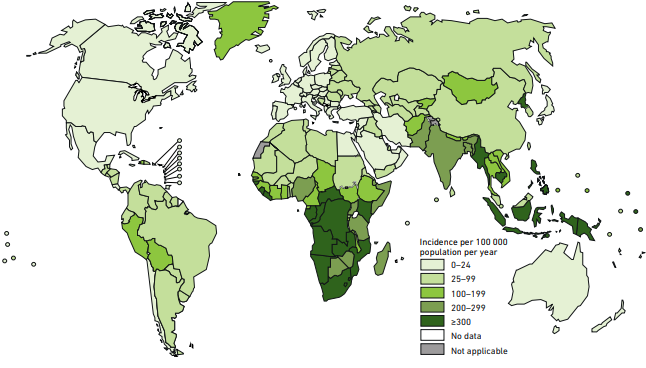
\includegraphics[width=\linewidth]{tb_incidence_rates_2017.png}
 \caption{Estimated TB incidence rates, 2017 \cite{TBT:3}}
 \label{tb_incidence_rates_2017}
\end{figure}
\section{Pulmonary Tuberculosis}
\paragraph{}
Pulmonary TB is caused by the bacterium Mycobacterium tuberculosis (M tuberculosis). It affects the lungs and it may spread to other organs. Pulmonary \ac{tb} is highly contagious as a person may get \ac{tb} by breathing in air droplets of an infected person \cite{TBT:4}.
\section{Types of Pulmonary Tuberculosis}
\paragraph{}
There exist five types of pulmonary tuberculosis namely (infiltrating, focal, tuberculoma, miliary and fibro-cavernous). A 2D slice of CT scan for each type of pulmonary \ac{tb} is shown in Figure \ref{fig:tb_types}.
\paragraph{Miliary \ac{tb}}
Miliary tuberculosis (TB) is the widespread dissemination of Mycobacterium tuberculosis via hematogenous spread. Classic miliary TB is defined as millet-like (mean, 2 mm; range, 1-5 mm) seeding of TB bacilli in the lung, as evidenced on chest radiography. This pattern is seen in 1-3\% of all TB cases.
Symptoms may include fever, night sweats, and weight loss. It can be difficult to diagnose because the initial chest x-ray may be normal. Patients who are immunosuppressed and children who have been exposed to the bacteria are at high risk for developing miliary TB.\cite{TBMIL:1,TBMIL:2,TBMIL:3, TBMIL:4}
\paragraph{Focal \ac{tb}}
Focal TB is diagnosed in the event of lesions not exceeding two lung segments. A small number of pathological foci with a diameter of about 1 cm are formed in the lung, which occurs at different times.\cite{TBFOC:1}
\paragraph{Infiltrative Tuberculosis}
infiltrative tuberculosis is characterized by the fuzzy outlines of shadows on radiography. This often happens when forming new cavities. infiltration appears on radiography as rounded, or shade of homogeneous structure. All spots are divided into small, medium and large. The small ones have a size of 1 to 2 cm, the means 2-4 cm, the large ones up to 6 cm.\cite{TBINF:1}
\paragraph{Tuberculoma \ac{tb}}
A tuberculoma is a clinical manifestation of tuberculosis which unites tubercles into a solid chunk, and so can mimic cancer tumors of many types in medical imaging studies.\cite{TBTUM:1,TBTUM:2}
\paragraph{Fibrous-cavernous \ac{tb}}
Distinctive features of cavernous form of lung tuberculosis are the presence of the thin-walled cavity located on a background of slightly changed lung tissue at absence of the expressed infiltrative and fibrotic changes. Cavernous tuberculosis develops among patients with, disseminated, focus lung tuberculosis, at disintegration of tuberculomas; at late revealing of disease, when the phase of disintegration is finished by formation of cavities, and the attributes of the initial form disappear. At radiographic examination rounded cavity is defined, with a thin two-layer wall and usual localization in subclavicular area.\cite{TBFIB:1}
\begin{figure}[h!]
  \centering
  \begin{subfigure}[b]{0.3\linewidth}
    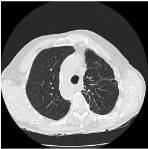
\includegraphics[width=\linewidth]{infiltrative.png}
    \caption{Infiltrative}
  \end{subfigure}
  \begin{subfigure}[b]{0.3\linewidth}
    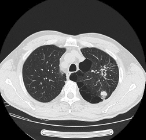
\includegraphics[width=\linewidth]{focal.png}
    \caption{Focal}
  \end{subfigure}
  \begin{subfigure}[b]{0.3\linewidth}
    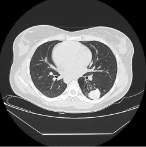
\includegraphics[width=\linewidth]{tuberculoma.png}
    \caption{Tuberculoma}
  \end{subfigure}
  \begin{subfigure}[b]{0.3\linewidth}
    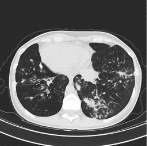
\includegraphics[width=\linewidth]{miliary.png}
    \caption{Miliary}
  \end{subfigure}
  \begin{subfigure}[b]{0.3\linewidth}
    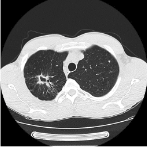
\includegraphics[width=\linewidth]{fibro-cavernous.png}
    \caption{Fibro-cavernous}
  \end{subfigure}
  
  \caption{CT slices of the five pulmonary \ac{tb} types.\cite{ImageCLEF:1}}
  \label{fig:tb_types}
\end{figure}

\subsection{Summary}
\paragraph{}
As shown in this chapter, tuberculosis is a chronic and may result in the death of the infected person. Furthermore, \acs{tb} has several types that are diagnosed and treated diffrently. In the next chapter, the diffrent medical imaging technologies used to diagnose \acs{tb} are presented along with the role of machine learning to analyse medical imaging. A particular focus will be put on deep learning and its architectures and diffrent evaluation metrics.